\section{Background and related works}
This section gives the necessary insights about a typical GPU architecture,
 performance-related considerations, and differences between compute capabilities
  from CUDA perspective, as well as known approaches for memory optimizations, 
  while also providing the insights about partial evaluation and its known practical 
  applications.
\subsection{Nvidia CUDA}
Modern GPUs are highly parallel computational 
devices equipped with a very high-bandwidth memory, 
designed to speed up general-purpose computations. 
CUDA defines a specific programming model\footnote{\url{https://docs.nvidia.com/pdf/CUDA_C_Programming_Guide.pdf} \\
 (last accessed date: 30.05.2020)} and architecture 
 for NVIDIA GPUs. These details are provided considering Nvidia Tesla T4 GPU.
\paragraph*{Hardware architecture}
Nvidia Tesla T4\footnote{\url{https://www.nvidia.com/content/dam/en-zz/Solutions/design-visualization/technologies/turing-architecture/NVIDIA-Turing-Architecture-Whitepaper.pdf} 
(last accessed date: 30.05.2020)} GPU is of Turing architecture and constitutes of five Graphics Processing Clusters (i.e. self-contained GPUs), each including four Texture Processing
 Clusters that incorporates two Streaming Multiprocessors (SM) each. Each SM is built up of four processing blocks, each including a warp\footnote{A batch of 32 CUDA threads} scheduler, 
 dispatch unit, and units for a memory fetch, integer, and floating-point operations, latter being called CUDA-cores. The GPU includes 2560 of such cores. Further, Tesla is supplied with 16GB GDDR6 
 memory that supports throughput up to 320GB/s. Unlike previous architectures it incorporates shared memory in L1 cache, increasing the bandwidth up to 2x, and adds an independent integer datapath, 
 enabling concurrent execution of integer and floating-point operations. Finally, Tensor Cores has been introduced, being specialized execution units specifically for performing the tensor/matrix operations.

\paragraph*{Programing model}
CUDA implies Single Instruction Multiple Threads architecture, where each instruction is concurrently executed by multiple threads, that are combined in blocks, that populates a grid. Threads in a 
block are split into warps, which are distributed between warp schedulers on a single SM, such schedulers assign per-thread instructions to the available computation units. Hence, in general, threads
 in a warp should execute the same instruction to achieve the best performance, in case of different instructions, caused e.g. by an if-statement, the execution is serialized, this is called a \emph{thread-divergence}.
  A piece of a program that is intended to be executed on a GPU is called a device kernel and usually is implemented in CUDA C, where grid and block sizes also could be specified.

\begin{figure}[h!]
    \centering
    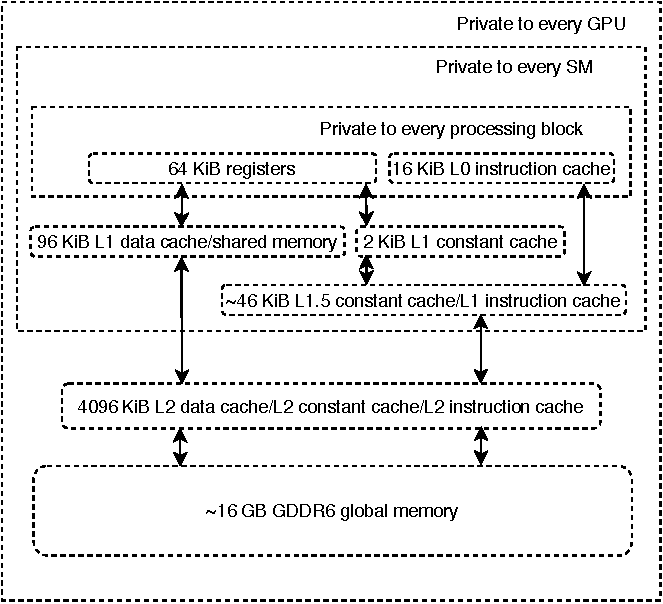
\includegraphics[width=\linewidth]{figures/TeslaT4Mem.pdf}
    \caption{Nvidia Tesla T4 memory hierarchy~\cite{TeslaT4Bench}}
    \label{fig:t4_mem}
\end{figure}

\paragraph*{Memory hierarchy}
Any GPU incorporates several memory types, that serve different purposes 
and differ in access latency, size, and bandwidth.
The memory architecture of Tesla T4 is depicted in \ref{fig:t4_mem}.

\emph{Global memory} is the main resource to transfer data between host and 
device. It is the largest and the slowest memory space, cacheable in L1 and L2 
caches, that have 32 B and 64 B lines respectively.
Global memory loads and stores by threads of a warp are served by the device 
with 32 B transactions\footnote{\url{https://docs.nvidia.com/cuda/pdf/CUDA\_C\_Best\_Practices\_Guide.pdf} 
(last accessed date: 30.05.2020)}.
Basically, concurrent accesses of the threads in a warp will coalesce into a 
number of such transactions necessary to service all the threads in the warp.
So in order to keep the number of such transactions to a minimum, threads in 
a warp should access adjacent segments of memory, aligned with the transaction 
size, avoiding strided accesses.
Such a requirement could not always be satisfied in practice, thus GPU 
resources being used not to its maximum. This memory space is accessible and 
allocated from the host, and visible to all the threads in a grid. 

\emph{Shared memory} is on-chip memory (hence it has lower latency and higher 
bandwidth than global memory) used to optimize frequent accesses to the same 
elements in global memory.
It is fast as long as bank conflicts do not occur.
The whole shared memory space is divided into 32 banks --- 4 B memory elements, 
with successive 4 B words belonging to successive banks. 
Any bank has a bandwidth of 4 B per clock cycle.
Therefore, any memory load or store of $n$ addresses, belonging to $n$ distinct 
memory banks
could be serviced simultaneously with the bandwidth of $n$ times the bandwidth 
of a single bank.
However, accesses to memory addresses from the same bank are serialized, 
decreasing the effective bandwidth in a magnitude of the number of conflict-free accesses. 
When multiple threads of a warp access the same shared memory, a broadcast occurs. Several 
such broadcasts could coalesce into a single multicast. This memory space has a visibility 
scope of a single thread block and is not accessible from the host.

\emph{Constant memory} is a cacheable off-chip memory, that is read-only from the device. 
It is a 64 KB part of global memory, that has a specific path for caching. As a result, 
on a cache miss, a constant memory read costs one memory read from global memory; otherwise, 
it is as fast as register access. When the threads in a warp access different constant memory addresses, 
these accesses are serialized.  Thus the constant cache is best when the threads in warp access the same 
or very few distinct addresses, in the first case the access is broadcasted, and the latency is the same 
as registers one.

\emph{Register memory} is on-chip memory, consuming zero extra clock cycles per instruction, as long as 
there is no register read-after-write dependencies and bank conflicts. Is has a scope of a single thread 
and is the fastest memory type available.


\subsection{Memory optimizations}
Given such a sophisticated memory hierarchy that should be managed by a programmer, memory optimizations 
are in a great interest. Only automatic memory optimizations would be considered, avoiding the guidelines 
about how to rearrange existing access patterns and speed-up the transferring between host and device.

In cases when abundant data parallelism is hard to achieve, e.g. when utilizing concurrent data structures 
and related synchronization primitives that arbitrate the accesses, dynamic memory allocation, i.e. per-thread allocation
 inside the device code, for such data structures becomes a bottleneck, hurting the throughput. In~\cite{NvidiaAllocator}
  a novel approach for dynamic memory allocation is proposed. It is based on shared data structures, supporting fine-grained
   mutual exclusion regions, cooperative synchronization primitives allowing to allocate memory concurrently between the threads,
    and a policy of execution delegation. The proposed allocator has a much higher allocation throughput compared to the one, deployed with CUDA.

Since the register memory is bounded in size, excessive registers\footnote{When the compiler needs more registers, than available on SM.} 
could be spilled into the global memory, introducing higher latency. 
Contrary to the default CUDA compiler approach, that handles excessive
 registers via re-materialization\footnote{Recomputation of a value instead 
 of loading and storing.
It produces the code with lower efficiency, however with lower register usage as well.} 
as long as possible before spilling, an approach from~\cite{RegisterSpilling} advocates 
the usage of underutilized shared memory to spill the excessive registers.
The approach is implemented as an extra binary translation pass over CUDA assembly.
Under certain conditions, such optimization is worse than CUDA default approach, thus 
the authors also provide a compile-time performance gain estimator, based on collected either explicit or implicit\footnote{Some stalls are labeled by the compiler, others are deduced, based e.g. on latencies for the memory type being accessed by the instruction.} instruction stalls, to compare the default code produced by the compiler and an optimized one, to decide which one is better.
On average, this technique achieves 10\% better performance on the selected benchmarks.

Another work is focused at the automatic allocation of shared memory to reduce the number of global memory transactions~\cite{AutomaticSharedMem} for automatically C-to-CUDA generated programs.
Authors propose a performance model, designed to choose the best configuration for shared memory allocation, considering estimated execution time, memory metrics, and the number of reduced global memory transactions.
Once the best configuration is found, it is applied
to the original C code by adding specific OpenACC\footnote{A set of directives for heterogeneous code parallelization} pragmas.

To tackle the problem of the lack of available GPU memory, a domain-oriented memory pooling and swapping is proposed in~\cite{zhang2019efficient}. Variables not in use are swapped to host and swapped back before any access, while variables that have non-overlapping lifetime could be allocated to the same memory space by the heuristic-driven memory pool. The heuristic is based on the iterative nature of the deep learning training algorithms to derive the lifetime and read/write order of all variables.

%тут бы переход какой-то к след подсекции
Despite such a variety of different memory optimization approaches, none of the presented works exploits possible static nature of device kernel parameters in any way. Thus, the application of partial evaluation technique to GPU kernels could provide another optimization approach, oriented at static data management.

\subsection{Partial evaluation}\label{PEsurvey}
%написать про partial evaluation с примером
\emph{Partial evaluation} is a program transformation and optimization technique, also known as program \emph{specialization}, first formulated in~\cite{Kleene1952-KLEITM}.
A partial evaluator is an algorithm, that takes a program and some of its known inputs called \emph{static} and produces another residual program, one yielding the same result given the remaining \emph{dynamic} inputs as the original program would have produced given all the inputs at once as illustrated in commutative diagram~\ref{fig:mix}.
A partial evaluator performs a mixture of code generation and execution: it reduces those parts of program \textbf{p}, depending on \textbf{in1}, and generates code for calculations for yet unavailable \textbf{in2}.
Generally, it performs symbolic computations, unfolding function calls, and replacement of function calls to their specialized versions.
For example, a partial evaluator for the program in listing~\ref{fig:pow} reduces the number of static conditional statements driven by static parameter. 

\begin{figure}
    \centering
    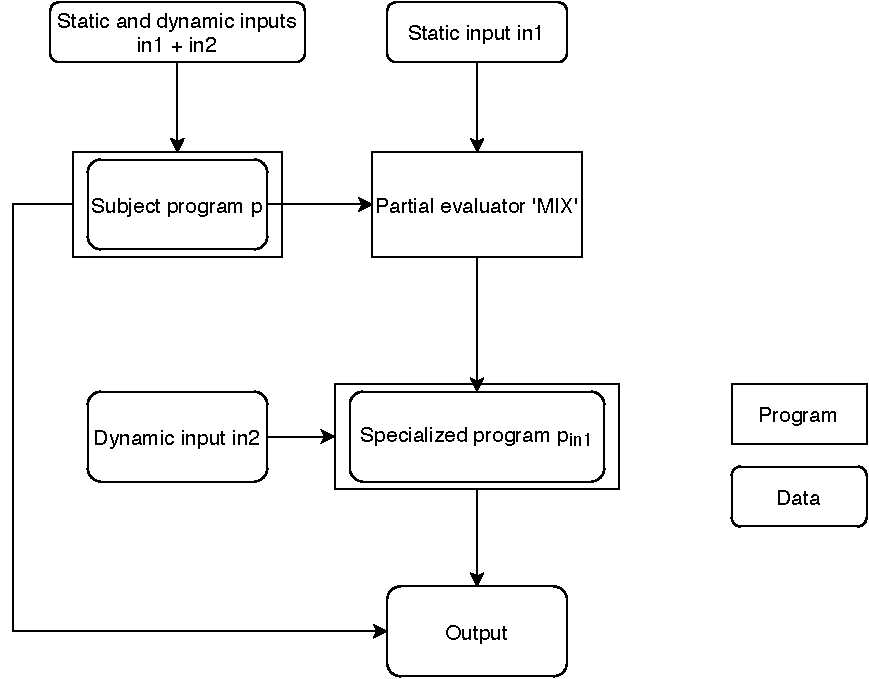
\includegraphics[width=0.85\linewidth]{figures/MixCommutativity.pdf}
    \caption{Partial evaluation pipeline}
    \label{fig:mix}
\end{figure}

The key idea is that a specialized program requires fewer computations (through moving them to compile or specialization time), and thus is intended to be more effective. A notable feature of specialization is the ability to generate a compiled program, once given an interpreter and a source program, also known as the first Futamura projection~\cite{Futamura1999}.
And while many practical applications benefit from partial evaluation through reducing the interpretation overhead (either by generating a compiler or exploiting interpretative nature of a program), there are scenarios, when a program takes more than one input, and one of the inputs varies more slowly than the others, thus specialization with respect to less-variable input could produce a more effective program.
Significant speed-up results were reported for pattern recognition, ray tracing, database querying, and scientific computing~\cite{Jones1993}.

\begin{listing}
    \begin{pyglist}[language=C,label=fig:pow,caption=Pow function partial evaluation example]
int pow(int x,int n){
    if (n == 0) return 1;
    else if (n % 2 == 0) { 
        return pow2(f(x,n/2));
    }
    else return x * f(x,n-1);
}
//partially evaluating pow(x,5) yields:
int pow(int x){
    return x * pow2(pow2(x));
}
    \end{pyglist}
\end{listing}


In~\cite{JavaPe} an annotation-driven partial evaluator for Java programming language is introduced.
The goal is to specialize framework configurations and quite expensive reflection calls, which are widespread in object-oriented systems. The replacement of reflective method calls with partially evaluated ordinary calls allows to speed-up a dynamic pricing system by a power of six.

In~\cite{SuperVm} an approach for automatic virtual machine construction is proposed, which allows new languages to be implemented through the specification of abstract syntax tree interpreter. Partial evaluation is used to compile hot and stable parts of the already specialized\footnote{Supplied with runtime information such as types.} interpreter.

Another usage of partial evaluation as a means for compilation has been described in~\cite{LLVMmix}. 
The PostgreSQL query interpreter, compiled at first to LLVM IR, which 
the designed partial evaluator works with, has been specialized in 
runtime with respect to the query, i.e. the query has been compiled. 
The approach results in rather significant performance improvement, 
requires fewer efforts compared to just-in-time compiler development 
and is fully automatic.


Despite such a rather broad variety of partial evaluation- related research, at the moment of writing, there is a lack of research combining GPGPU and partial evaluation.
In~\cite{JitGPUPE} the approach from~\cite{SuperVm} was adopted to compile code from \emph{R} language to \emph{OpenCL}, to make it possible to write GPU-accelerated applications with dynamic interpreted languages, popular in big data, ignoring third-party libraries and relatively low-level programming languages for GPU. A metaprogramming system for writing shaders is presented in~\cite{GPUsh}, which supports partial evaluation via currying. However, the system is rather outdated and has no relation to modern GPGPU programming. Furthermore, there are no works dedicated to what benefits partial evaluation could provide once applied directly to GPU program, or whether it could provide any at all.

\begin{listing}
    \begin{pyglist}[language=Java,label=fig:kernel,caption=A typical GPGPU kernel]
handleData (filterParams, data) {
    res = new List()
    for d in data
        for e in filterParams
            if d % e == 0 
            then res.Add(d)
    return res
}
        
    \end{pyglist}
\end{listing}


\begin{listing}
    \begin{pyglist}[language = Java, label = fig:kernel_mix,caption={ A typical GPGPU kernel specialization with respect to {[2;3]}}]
handleData_spec (data) {
    res = new List()
    for d in data
        if d % 2 == 0 ||
        d % 3 == 0
        then res.Add(d)
  return res
}
    \end{pyglist}
\end{listing}


However, in practice, it appears that many GPGPU scenarios could have static parameters in a sense, theoretically appropriate for specialization.
A typical GPGPU kernel is depicted in listing~\ref{fig:kernel}.
It often represents some kind of a filter, that is applied to different pieces of the data in parallel by a huge number of threads.
The execution time primarily depends on the size of the data, which often exceeds the available memory of GPU, therefore the device kernel is run multiple times on different chunks of the data, resulting in significant execution time.
Hence, the filter varies less frequently than the data and could be considered as a static input and subjected to specialization.
However, the filter becomes known at runtime, before the kernel actually runs, thus the specialization should be performed at runtime.
The overhead of the partial evaluation could be hidden by the gained speed-up across the long run of the kernel.
Moreover, since one filter could be applied to different data pieces, the specialized version could be cached and reused instead of specializing again. The effect of specialization could be seen in listing~\ref{fig:kernel_mix}.
The inner cycle with accesses to the memory space of the filter has been reduced with the filter parameters being placed directly into the instructions.
Since memory access operations have been proven to be the most expensive, such a replacement could provide a benefit of accessing the filter from the registers, which is the fastest memory type, rather than from any other memory space.
Furthermore, a partial evaluator could be able to reduce those parts of the kernel, that depend on static filter parameters made available.

\subsection{AnyDSL framework}
To the date of writing, there is no partial evaluator known that 
works directly with CUDA C or any of CUDA intermediate representations.
As mentioned, the partial evaluator from~\cite{LLVMmix} works with LLVM IR, and CUDA has 
an appropriate LLVM frontend, however, the partial evaluator leverages special 
attributes in IR, that conflicts with the ones of CUDA itself during LLVM JIT 
compilation.
AnyDSL~\cite{LeiBa} is a framework for the development of domain-specific 
libraries that could utilize different backends, including the one of CUDA.
The framework includes a partial evaluator that works with a specific intermediate 
representation, supporting CUDA C code generation.
The framework requires the programs to be developed in a special DSL named 
\emph{Impala}, which resembles C language with functions being the first-class 
objects.
Since the DSL is very CUDA C alike, the framework has been chosen as a means 
for partial evaluation of GPU programs.


\begin{listing}
    \begin{pyglist}[language=Rust, label = fig:impala_cuda, caption=Impala GPU-accelerated loop]
    fn iterate(fld: Field , @body: fn(int, int) -> ()) -> () {
        let grid = (fld.cols , fld.rows , 1);
        let block = (128 , 1, 1);
        cuda(grid , block , || {
            let x = tid_x() + blockDim_x() * blockId_x();
            let y = tid_y() + blockDim_y() * blockId_y ();
            body(x, y);
        });
    }
    \end{pyglist}
    \end{listing}

The impala compiler translates the code into a functional graph-based intermediate 
representation similar to typed lambda calculus with continuations. 
Such a representation allows Impala to achieve near C performance, 
despite higher-order functions support~\cite{Thorin}.
Partial evaluation is performed on this level, while the representation 
could target different hardware architectures utilizing LLVM and compiler 
intrinsics.
An example of such an intrinsic is given in listing~\ref{fig:impala_cuda}.
The whole function would be first converted into the intermediate representation, 
with the parts of the function labeled with \lstinline{@} 
partially evaluated, then the device-independent 
parts of the code would be translated into LLVM and device code 
would be translated into device-specific code, e.g. 
the code between lines 4-8 would be translated into CUDA C, 
which then would be included in LLVM code with a call to an external 
function that loads and executes the generated device code, 
e.g. the external function for mentioned lines would call NVIDIA CUDA 
compiler in runtime and launch the compiled kernel.



The authors of the framework evaluated the effectiveness of partial evaluation
 targeting different backends, including CUDA~\cite{LeiBa,OnlinePe}.
  The results show similar performance with hand-tuned third-party implementations.
   However, the authors focused on compile-time partial evaluation of kernels and
    have not provided any GPU-specific details that affect the success
     of the result as well as what particular optimization a partial evaluator
      performs with the device code.
       In contrast, this work is aimed at revealing GPU architecture details
        that affect the success of partial evaluation,
         focused at runtime partial evaluation and selects different
          experimental scenarios.

